\documentclass[12pt, a4paper]{article}
\usepackage[utf8]{inputenc}
\usepackage[IL2]{fontenc}
\usepackage[czech]{babel}

\usepackage[colorlinks=true]{hyperref}
\usepackage{graphicx}


%Nastavi hloubku obsahu \setcounter{tocdepth}{3}

\begin{document}
	\begin{titlepage}
		\begin{center}
			
\includegraphics{img/ZCULogo.pdf}\\[1cm]
			\textsc{\LARGE Západočeská univerzita v~Plzni}\\[0.1cm]
			\textsc{\Large Fakulta aplikovaných věd}\\[0.1cm]
			\textsc{\large Katedra informatiky a~výpočetní techniky}
			\vfill
			\textsc{\LARGE Semestrální práce KIV/UPS}\\[0.2cm]
			\Large{Síťová hra Oběšenec\\za použití protokolu UDP}
			\vfill
			Jaroslav Klaus\\
			A13B0347P\\
			jklaus@students.zcu.cz\\[0.2cm]
			\today, Plzeň
		\end{center}
	\end{titlepage}

	\tableofcontents
	\newpage

	\section{Zadání}
	Vytvořte hru, kterou může hrát více hráčů. Řešení musí obsahovat program serveru, který bude obsluhovat více klientů i her současně. Klient bude po opětovném přihlášení pokračovat tam, kde přestal. Program musí být odolný proti chybným zadáním a musí adekvátně reagovat na výpadky serveru i klientů. Klient bude naprogramován v jazyce \emph{Java} a server v jazyce \emph{C} nebo \emph{C++}. Konkrétně vytvořte hru \emph{Kvarteto} za použití protokolu \emph{TCP}.
	
	Program bude doplněn o zpracování statistických údajů (počet odeslaných a přijatých zpráv a bytů, počet přijatých spojení, počet spojení ukončených z důvodu chybných dat apod.). Dále nesmí chyby v komunikaci znemožnit případně znesnadnit používání grafického rozhraní klienta.
	
	\section{Popis hry}
	Hra Kvarteto je relativně jednoduchá. Jedná se o karetní hru, kterou je možné hrát ve třech a více hráčích (maximálně však 32). Hraje se s kartami označenými písmenem a číslem (1A, 1B, 1C, 1D, 2A, 2B, \dots, 8D). Cílem hry je získat čtveřici karet s příslušným číslem, např. 1A, 1B, 1C a 1D. Tah probíhá tak, že hráč některého ze soupeřů požádá o kartu, kterou potřebuje. Pokud ji soupeř má, předá ji hráči, který pokračuje dalším tahem. Pokud kartu soupeř nemá, je na tahu on.
	
	\section{Protokol}
	Protokol TCP je tzv. spolehlivý. Řeší za nás ztrátu zpráv během přenosu, jejich duplicitu, pořadí a další, proto není potřeba tyto stavy řešit. Důležité však je zjistit výpadek klienta, který řádně neukončil spojení. To je zajištěno periodickým posíláním zpráv \emph{\uv{keep-alive}}. Pokud od serveru nebo klient ta určité doby nedorazí tato zpráva, bude prohlášen za nedostupného a spojení s ním ukončeno.

	Komunikační protokol bude textový s oddělovačem \emph{';'}. Bude se skládat ze tří částí, viz tabulka \ref{Vzhled}. Data budou jako oddělovač používat \emph{','}. Zpráva bude ukončena znakem '\textbackslash n' nebo "\textbackslash r\textbackslash n" (v závislosti na použitém OS). Vzhledem k tomu platí pro data (přezdívky, id her apod.) omezení, že nesmí obsahovat tyto vyhrazené znaky. Zpráva tedy může vypadat např. takto: "5;6;nick,3\textbackslash n".
		\begin{table}[ht!]
			\centering
			\caption{Vzhled zprávy}
			\label{Vzhled}
			\begin{tabular}{| c | c | c |}
				\hline
				typ zprávy & velikost dat & data\\
				\hline
			\end{tabular}
		\end{table}
	
	\subsection{Typy zpráv a dat}
	Typ zprávy bude uveden číslem, u kterého bude dále popsán význam a naznačeno, jak budou vypadat data. Jako první v popisu bude uvedeno, zda se jedná o zprávu od klienta na server (C), nebo od severu ke klientovi (S).
		\begin{enumerate}
		\setcounter{enumi}{-1}
		\item S, C, \textbf{keep-alive}\\
		Data: -
		
		\item C, \textbf{žádost o seznam her}\\
		Data: -
		
		\item S, \textbf{seznam her}\\
		Data: počet her (int)\\
			\null \quad seznam her [\\
			\null \qquad id hry (string)\\
			\null \qquad počet připojených (int)\\
			\null \qquad kapacita (int)\\
			\null \quad ]
			
		\item C, \textbf{žádost o připojení}\\
		Data: jméno (string)\\
			\null \quad id hry (string)
			
		\item S, \textbf{odpověď na žádost o připojení}\\
		Data: 0 pokud vše proběhlo v pořádku\\
			\null \quad 1 pokud je hra plná\\
			\null \quad 2 pokud je hráč již na serveru\\
			\null \quad 3 pokud již hra neexistuje
			
		\item C, \textbf{žádost o vytvoření hry}\\
		Data: jméno (string)\\
			\null \quad počet soupeřů (int)
		
		\item S, \textbf{odpověď na žádost o vytvoření hry}\\
		Data: 0 pokud vše proběhlo v pořádku\\
			\null \quad 1 pokud je hráč již na serveru\\
			\null \quad 2 pokud bylo zadáno moc málo hráčů
		
		\item S, \textbf{začátek hry}\\
		Data: počet soupeřů (int)\\
			\null \quad pro každého protihráče [\\
			\null \qquad jméno (string)\\
			\null \qquad počet karet (int)\\
			\null \quad ]\\
			\null \quad počet mých karet (int)\\
			\null \quad seznam mých karet [\\
			\null \qquad karta (string)\\
			\null \quad ]
		
		\item S, \textbf{jsi na tahu}\\
		Data: -
		
		\item S, \textbf{oznámení, kdo je na tahu} (pro ostatní hráče)\\
		Data: jméno (string)
		
		\item C, \textbf{tah}\\
		Data: protihráč (string)\\
			\null \quad požadovaná karta (string)

		\item S, \textbf{odpověď na tah}\\
		Data: 0 pokud kartu vlastní\\
			\null \quad 1 pokud kartu nevlastní

		\item S, \textbf{oznámení tahu} (pro ostatní hráče)\\
		Data: výsledek tahu (\\
			\null \qquad 0 pokud kartu vlastnil\\
			\null \qquad 1 pokud kartu nevlastnil\\
			\null \quad )\\
			\null \quad jméno (string)\\
			\null \quad karta (string)\\
			\null \quad protihráč (string)

		\item S, \textbf{vyhrál jsi} (= konec hry, má kvarteto)\\
		Data: -

		\item S, \textbf{oznámení o někom, kdo vyhrál} (pro ostatní hráče)\\
		Data: jméno (string)

		\item S, \textbf{prohrál jsi} (= konec hry, nemá žádnou kartu)\\
		Data: -

		\item S, \textbf{oznámení o někom, kdo prohrál}\\
		Data: jméno (string)

		\item S, \textbf{ukončení hry z důvodu nedostupnosti hráče}\\
		Data: jméno (string)

		\item C, \textbf{žádost o navázání přerušené hry}\\
		Data: jméno (string)

		\item S, \textbf{odpověď na žádost o navázání přerušené hry}\\
		Data: výsledek (\\
			\null \qquad 0 pokud vše proběhlo v pořádku, následují data\\
			\null \qquad 1 pokud hráč nebyl na serveru nalezen\\
			\null \qquad 2 pokud byl nalezen, ale je aktivní\\
			\null \qquad pokud vše proběhlo v pořádku, ale hra ještě nezačala\\
			\null \quad )\\
			\null \quad počet soupeřů (int)\\
			\null \quad pro každého protihráče [\\
			\null \qquad jméno (string)\\
			\null \qquad počet karet (int)\\
			\null \quad ]\\
			\null \quad počet mých karet (int)\\
			\null \quad seznam mých karet [\\
			\null \qquad karta (string)\\
			\null \quad ]

		\item C, \textbf{odpojuji se}\\
		Data: -
		\end{enumerate}
		
	\subsection{Posloupnost zpráv v bezproblémové hře}
		Každých 2500 milisekund zpráva \emph{"0;0;"} od klienta i serveru.
		
		Po navázání spojení může vypadat komunikace např. takto:\\
		C: 1;0;\\
		S: 2;1;0\\
		C: 5;6;nick,2\\
		S: 6;1;0\\
		S: 7;55;2,enemy1,11,enemy2,10,11,1A,2B,3C,4B,4D,5A,6B,7C,8D,5C,2D\\
		S: 8;0;\\
		C: 10;9;enemy1,2A\\
		S: 11;1;1\\
		S: 9;6;enemy1\\
		S: 12;16;0,enemy1,1A,nick\\
		S: 14;6;enemy1
		
	\section{Implementace}
	Zde je popsána dekompozice, rozvrstvení, metoda paralelizace a další implementační záležitosti programů.
	
		\subsection{Server}
		Server je rozdělen do čtyř hlavních částí. První část je zpracování požadavků klientů, kteří nejsou v žádné hře. Druhou částí je management hry a jejích klientů. Třetí část slouží k periodickému zasílání \uv{keep-alive} zpráv všem klientům na serveru. Konečně čtvrtá část slouží ke kontrole, zda jsou klienti dostupní (posílají \uv{keep-alive} zprávy), a k případnému ukončení spojení s těmi nedostupnými. Každá z těchto částí běží ve vlastním vlákně, přičemž každá hra má vlákno vlastní.
		
			\subsubsection{Klienti mimo hru}
			Tato část volá funkci \emph{select} s krátkým timeoutem nad sockety klientů mimo hru a serveru. Pokud se zjistí, že na některém z klientských socketů jsou data ke čtení, provede se jejich načtení a zpracování. Pokud se něco událo na socketu serveru, je přijato nové spojení s klientem. Typy zpráv, které budou zpracovány v této části jsou: 0, 1, 3, 5 a 18. Zde probíhá vytváření her, připojení klientů do her apod.
			
			\subsubsection{Management hry}
			Tato část volá funkci \emph{select} s krátkým timeoutem nad sockety klientů ve hře. Pokud se zjistí, že na některém z klientských socketů jsou data ke čtení, provede se jejich načtení a zpracování. Typy zpráv, které budou zpracovány v této části jsou: 0, 10 a 20. Zde probíhá management hry jako je rozdání karet, kontrola tahů apod.
			
			\subsubsection{Periodické zasílání \uv{keep-alive}}
			Tato část prochází seznamy klientů mimo hry i ve hrách a každému pošle zprávu typu \uv{keep-alive}a poté se na 2500 milisekund vlákno uspí. Toto je jediná funkce této části.
			
			\subsubsection{Kontrola dostupnosti klientů}
			V tomto vlákně se prochází seznamy klientů mimo hry i ve hrách. U každého se kontroluje čas poslední přijaté zprávy \uv{keep-alive}. Pokud je tento čas starší než 5 sekund, nastaví se stav hráče jako neaktivní a je tak možné, aby klient požádal o navázání přerušené hry (pokud v nějaké byl). Pokud je čas starší než 25 sekund, je spojení s klientem ukončeno a případná hra ukončena z důvodu nedostupnosti hráče.
		
		\subsection{Klient}
		Postup práce klienta je téměř identický jako ten na serveru. Liší se např. v tom, že zde existuje pouze jedno vlákno pro příjem a zpracování zpráv. Další vlákno slouží pro odesílání zpráv \uv{keep-alive}, jiné pro kontrolu dostupnosti serveru a poslední k ovládání GUI.
		
	\section{Uživatelská příručka}
		\subsection{Server}
		Server je napsán v jazyce \emph{C++} v operačním systému Linux a je k němu vytvořen příslušný \emph{Makefile}, kterým je možné server pomocí nástroje \emph{make} jednoduše přeložit. K přeložení je potřebná knihovna \emph{pthread} pro možnost vytvoření a práce s vlákny a knhovna \emph{uuid} pro vytváření id her. Server se spouští se dvěma parametry, adresou pro naslouchání a portem, např.:\\
		\texttt{./QuartetteServer INADDR\_ANY 10000}\\
		Ukončení serveru je možné provést zasláním signálu \emph{SIGINT} (např. stisknutí Ctrl + C).
	
		\subsection{Klient}
		Klient je napsán v jazyce \emph{Java} za použití \emph{JavaFX} a \emph{JDK 8} a fungovat by měl jak v OS Linux, tak Microsoft Windows. Pro jeho přeložení je potřeba \emph{JDK 8} nebo vyšší, pro spuštění by měl stačit \emph{JRE 8} nebo vyšší. Přiložen je soubor \emph{pom.xml} pro automatický překlad nástrojem \emph{maven}, který se provede např. příkazem:\\
		\texttt{mvn package}\\
		Vytvoří se soubor \emph{QuartetteClient.jar}, který lze spustit např. příkazem:\\
		\texttt{java -jar QuartetteClient.jar}\\
		Je možné spustit klienta s parametry, které předvyplní daná pole, např. takto:\\
		\texttt{java -jar QuartetteClient.jar -host localhost}\\
		\texttt{java -jar QuartetteClient.jar -port 10000}\\
		\texttt{java -jar QuartetteClient.jar -nick nick}, případně jejich kombinací.
		
		Po spuštění je požadováno zadání adresy a portu serveru, viz obrázek \ref{Login}. Po připojení se zobrazí menu jako na obrázku \ref{Menu}. Seznam her se zobrazí po kliknutí na příslušné tlačítko a vypadá jako na obrázku \ref{List}. Novou hru vytvoříme kliknutím na příslušné tlačítko a do dialogu \ref{NewGame} zadáme svou přezdívku a počet protihráčů. Hra vypadá jako na obrázku \ref{Game}. Obsahuje seznam protihráčů, vašich karet a historii.Ovládá se tak, že vyberete z nabídky protihráče, od kterého chcete kartu. Pokud jste na řadě, objeví se dialog, ve kterém vyberete kartu, kterou chcete. Pokud se ze hry odpojíte nekorektně, máte v blízké době šanci se do ní opět vrátit pomocí příslušného tlačítka v menu. To otevře dialog, kam zadáte svou původní přezdívku a budete vráceni do hry.
		
	\section{Závěr}
	Vytvoření zabralo o něco více času, než jsem očekával, cca 80 až 90 hodin. Jedním z důvodů bylo to, že nebylo jednoduché správně dekomponovat problém a uvědomit si všechny možné problémy a situace, které mohou nastat. Další překážkou byl jazyk, ve kterém musel být server implementován.
	
	V práci jsem navrhl komunikační protokol a vzhled zpráv, stavové diagramy servery, hry a hráče, implementoval a otestoval program klienta i serveru. Zadaní se mi tak, dle mého názoru, podařilo splnit.
	
	\begin{figure}[ht!]
		\centering
		\caption{Připojení k serveru}
		\label{Login}
		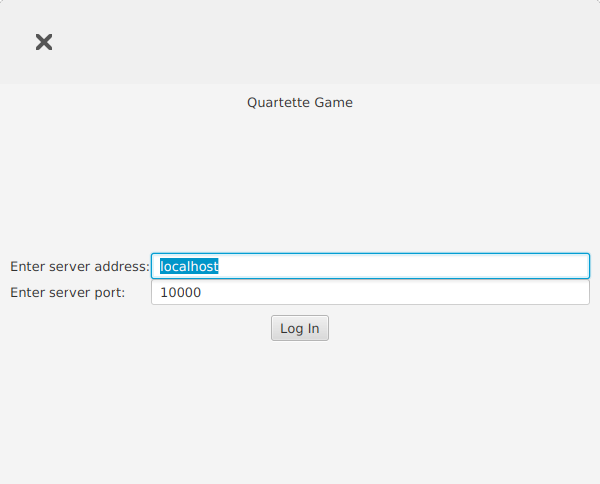
\includegraphics[width=11cm]{img/Login.png}
	\end{figure}
	\begin{figure}[ht!]
		\centering
		\caption{Menu hry}
		\label{Menu}
		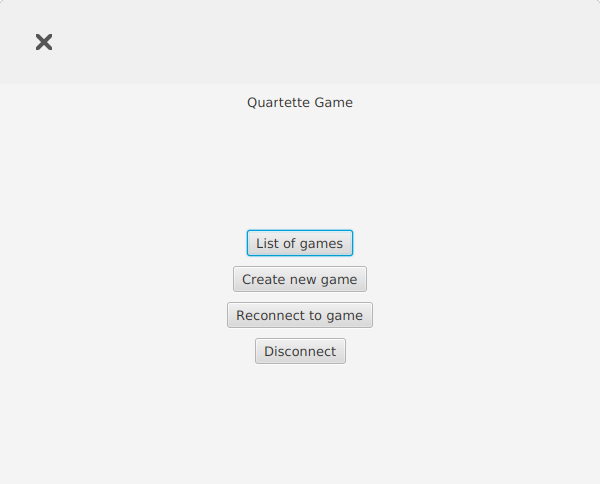
\includegraphics[width=11cm]{img/Menu.png}
	\end{figure}
	\begin{figure}[ht!]
		\centering
		\caption{Seznam her}
		\label{List}
		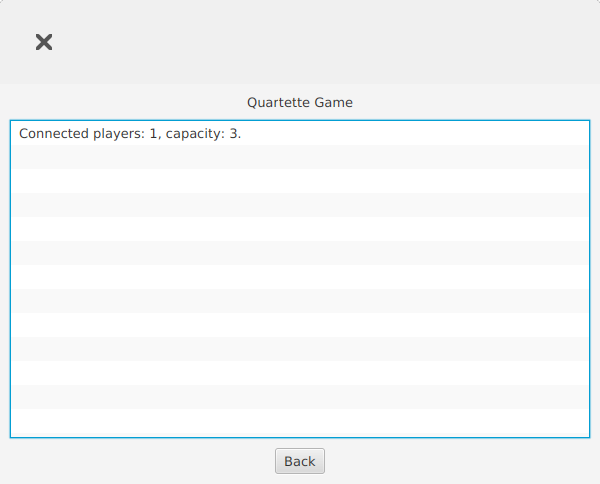
\includegraphics[width=11cm]{img/List.png}
	\end{figure}
	\begin{figure}[ht!]
		\centering
		\caption{Vytvoření nové hry}
		\label{NewGame}
		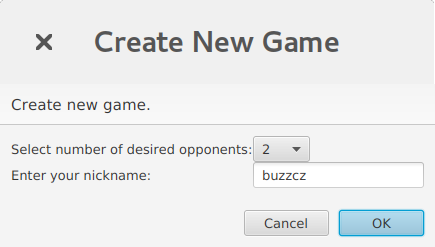
\includegraphics[width=11cm]{img/NewGame.png}
	\end{figure}
	\begin{figure}[ht!]
		\centering
		\caption{Hra}
		\label{Game}
		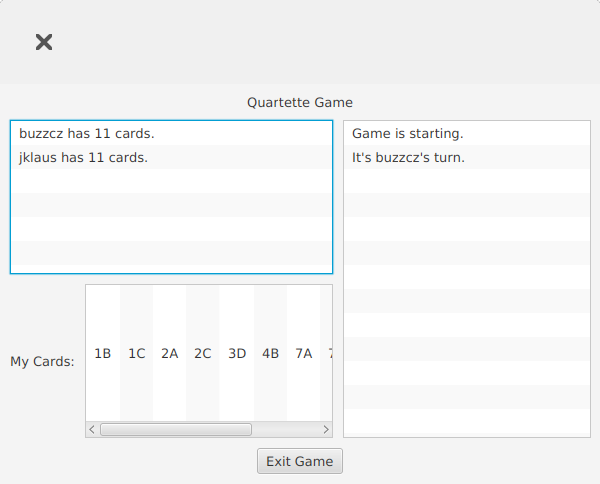
\includegraphics[width=11cm]{img/Game.png}
	\end{figure}
	
\end{document}